\section{Tuning a Kalman filter}

\subsection{a}

The model is :
\begin{equation}
    \begin{aligned}
        y_k^v=C(v_k+r_k^v)
    \end{aligned}
\end{equation}

From the model we can get:

\begin{equation}
    \begin{aligned}
        mean(y)&= C*mean(v_k)+C*mean(r_k)\\
        var(y) &= C^2*var(r_k) 
    \end{aligned}
    \label{eq2}
\end{equation}

Base on equation \ref{eq2}, we can get three diffent value of $ C $ and then calculate the final mean of $C$ by calculating the average mean of $C$:

\begin{lstlisting}
    data=[CalibrationSequenceVelocity_v0;CalibrationSequenceVelocity_v10;CalibrationSequenceVelocity_v20];
    meanv0 = mean(data(1,:));%c*mean(rk)
    meanv10 = mean(data(2,:));%c*10+c*mean(rk)
    meanv20 = mean(data(3,:));%c*20+c*mean(rk)
    C(1)=(meanv10-meanv0)/10
    C(2)=(meanv20-meanv10)/10
    C(3)=(meanv20-meanv0)/20
    C=mean(C)
\end{lstlisting}

Still according to equation \ref{eq2}, get covariance of $r_k$ by calculating the average mean $r_k$:

\begin{lstlisting}
    for i =1:3
    meanv(i) = mean(data(i,:));
    cov(i) = var(data(i,:))/C^2
    end

    P_r = mean(cov)
\end{lstlisting}

The final results are:

\begin{equation}
    \begin{aligned}
        C &= 1.1059\\
        P_r &=\text{Var}[r_k^v]= 2.4702
    \end{aligned}
\end{equation}

\subsection{b}

I have come up with two ideas to solve the lack of $Y_{position} $ problem.

The first one is to use prediction to fix the lack of $ Y_{position} $.To be detailed, if there is only a speed measurement available, use the predicted state estimate to estimate the position and update the state estimate and covariance matrix based on the estimated position and the speed measurement.

This method may make some sense because it can use every $ Y_{velocity} $, but the missing data is replaced with estimated values, in which way imputing missing data may introduce bias or other errors in the analysis.

The second method is to skip the $ Y $ data couple if the $ Y_{position} $ is missing. In this way, we will lose half of the $ Y_{velocity} $ but it does not have the risk of introducing unnecessary perturbations.

Finally, I applied the second method, and create my \texttt{kalmanFilterfusedskip} function below:

\begin{lstlisting}
    function [X, P,v] = kalmanFilterfusedskip(Y, x_0, P_0, A, Q, H, R, N)
    N = size(Y,2);
    
    n = length(x_0);
    m = size(Y,1);
    
    % Initialize state estimate and covariance
    X(:,1) = x_0;
    P(:,:,1) = P_0;
    
    for i=1:N
        % Prediction step
        [prex, preP] = linearPrediction(X(:,i), P(:,:,i), A, Q);
    
        if ~isnan(Y(1,i)) % Check if position measurement is available
            % Update step
            [X(:,i+1), P(:,:,i+1),v(:,i)] = linearUpdate(prex, preP, Y(:,i), H, R);
        else
            % Skip update step if position measurement is missing
            v(:,i)=0;
            X(:,i+1) = prex;
            P(:,:,i+1) = preP;
        end
    end
    
    % Remove the first element of X and P (the initial state estimate and covariance)
    X = X(:,2:end);
    P = P(:,:,2:end);
    v=v(:,1:2:end);
    end
    
\end{lstlisting}

\subsection{c}

For \texttt{CV model}, the matrice are define like this:

\begin{lstlisting}
    A=[1 Ts;0 1];%A for state update
    H=[1 0; 0 C]; %H for y=Hx
    Qcon=1;
    R=diag([Qcon C^2*cov_rvk]);%noise covariance for measurement
    % R=diag([16 16]);
    gamacv=[0;1];
    Qc=0.0001;%covariance of continuous time motion update
    Q=gamacv*Qc*gamacv';%discrete time covariance, motion
    x_0=[0 0]'; % just for prior, set it myself
    P_0=diag([10 10]);%just for prior , set it myself
\end{lstlisting}

For \texttt{CA model}, the matrice are define like this:

\begin{lstlisting}
    Aca = [1 Ts Ts^2/2;0 1 Ts;0 0 1];
    Hca = [1 0 0; 0 C 0;];
    gamaca=[0;0;1];
    Qca=gamaca*Qc*gamaca';%discrete time covariance, motion
    x_0ca=[0 0 0]'; % just for prior, set it myself
    P_0ca=diag([10 10 10]);%just for prior , set it myself
\end{lstlisting}

In the matrice above, the most important value that affects our results the most is $Qc$. The bigger the $Qc$, the more we believe in the measurement. The smaller the $Qc$, the more we believe in the process.

Also, the prior affects something, especially in the beginning part of the results. But as the same result from scenario 1, after enough process, the estimate will converge to the true estimate that because our step is 2000 that these priors do not matter at all.

It can not tell from the plot when $ Qc $ is within 1 to 4, so I set $ Qc $ to some extreme value to see the difference:

\begin{figure}[H]
    \centering
    \begin{subfigure}[b]{0.3\textwidth}
        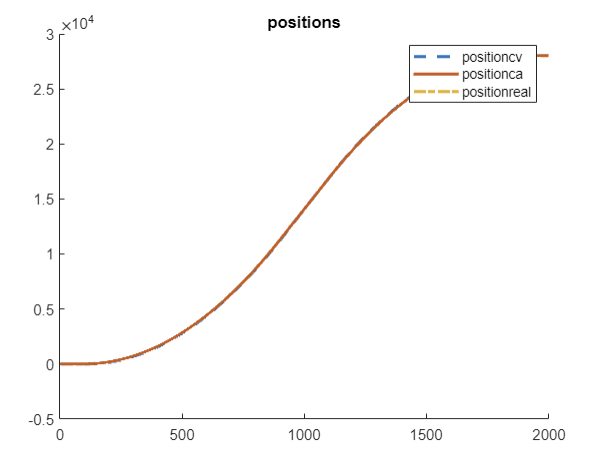
\includegraphics[width=\textwidth]{images/positionQc=0.0001.png}
        \caption{positionQc=0.0001}
        \label{fig:positionQc=0.0001}
    \end{subfigure}
    \begin{subfigure}[b]{0.3\textwidth}
        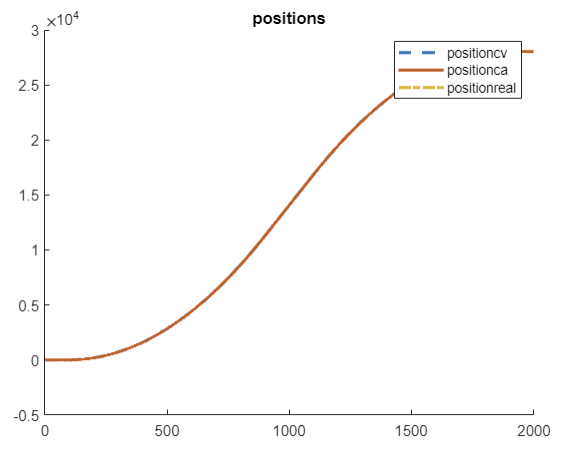
\includegraphics[width=\textwidth]{images/positionQc=1.png}
        \caption{positionQc=1}
        \label{fig:positionQc=1}
    \end{subfigure}
    \begin{subfigure}[b]{0.3\textwidth}
        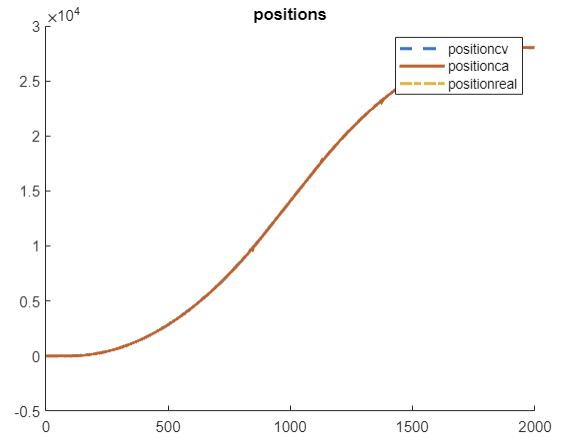
\includegraphics[width=\textwidth]{images/positionQc=10000.png}
        \caption{positionQc=10000}
        \label{fig:positionQc=10000}
    \end{subfigure}
    \caption{Change Qc and Observe Position curves}
    \label{21}
\end{figure}

\begin{figure}[H]
    \centering
    \begin{subfigure}[b]{0.3\textwidth}
        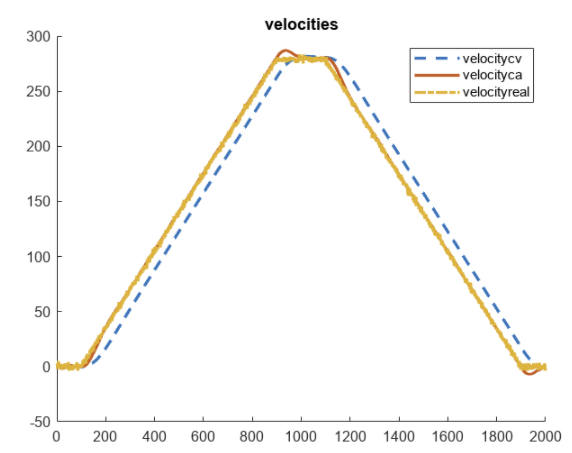
\includegraphics[width=\textwidth]{images/velocityQc=0.0001.png}
        \caption{velocityQc=0.0001}
        \label{velocityQc=0.0001}
    \end{subfigure}
    \begin{subfigure}[b]{0.3\textwidth}
        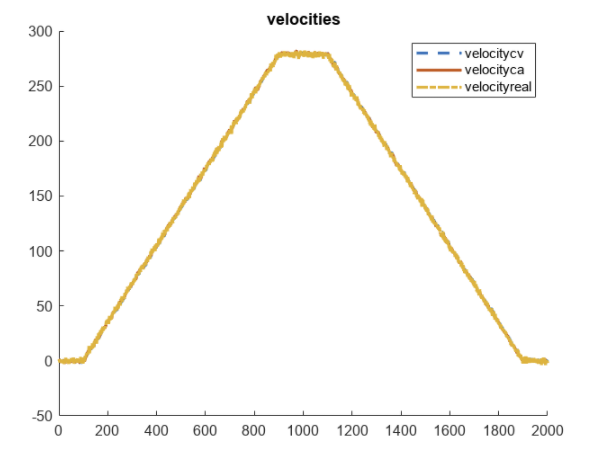
\includegraphics[width=\textwidth]{images/velocityQc=1.png}
        \caption{velocityQc=1}
        \label{fig:velocityQc=1}
    \end{subfigure}
    \begin{subfigure}[b]{0.3\textwidth}
        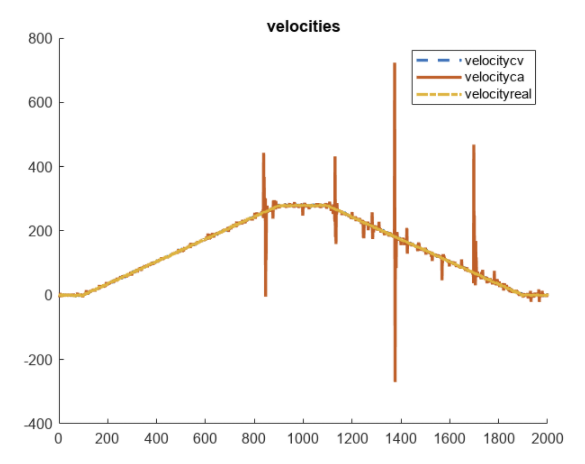
\includegraphics[width=\textwidth]{images/velocityQc=10000.png}
        \caption{velocity when Qc=10000}
        \label{velocityQc=10000}
    \end{subfigure}
    \caption{Change Qc and Observe Velocity curves}
    \label{22}
\end{figure}

From figure \ref{22}, the change of $Qc$ mainly affects the velocity prediction of both models.

After attempts, the best strategy is to keep $ Qc $ around a small value, which means the model believes more in the process, then the curves of both models converge to the real values.

\subsection{d}

After tuning the constant velocity (CV) and constant acceleration (CA) models and comparing their performance, it appears that the \texttt{CA model} performs better in this scenario.\\

\begin{table}[h]
    \centering
    \begin{tabular}{|p{0.45\linewidth}|p{0.45\linewidth}|}
    \hline
    \textbf{Advantages of CV model} & \textbf{Disadvantages of CV model} \\
    \hline
    Simpler model with fewer parameters to tune & May not perform well in scenarios where the acceleration of the object being tracked is changing rapidly \\
    \hline
    Suitable for scenarios where the acceleration of the object being tracked is assumed to be constant & May not accurately capture sudden changes in velocity or direction \\
    \hline
    Smoother estimates of the position and velocity & \\
    \hline
    \end{tabular}
    \caption{Advantages and disadvantages of the CV model}
    \end{table}


    \begin{table}[h]
        \centering
        \begin{tabular}{|p{0.45\linewidth}|p{0.45\linewidth}|}
        \hline
        \textbf{Advantages of CA Model} & \textbf{Disadvantages of CA Model} \\
        \hline
        Can capture rapid changes in acceleration and velocity & More complex model with more parameters to tune \\
        \hline
        More flexible model that can handle varying acceleration scenarios & May produce noisier estimates due to the increased complexity \\
        \hline
        \end{tabular}
        \caption{Advantages and disadvantages of the CA model.}
        \end{table}

In this scenario, from the true state value we can see the train is assumed to have constant acceleration, so the \texttt{CA model} performs better than the \texttt{CV model}. 

As for the quantitative analysis, I have calculated the corresponding $vk$ inside the code, which can be used to analyze the quality of the corresponding model through the \texttt{autocorr} function. The result are ploted as figure \ref{2d1} and figure \ref{2d2}, from which it is obvious that the \texttt{CA model} has better estimate quality in this scenario.

\begin{figure}[H]
 \centering
 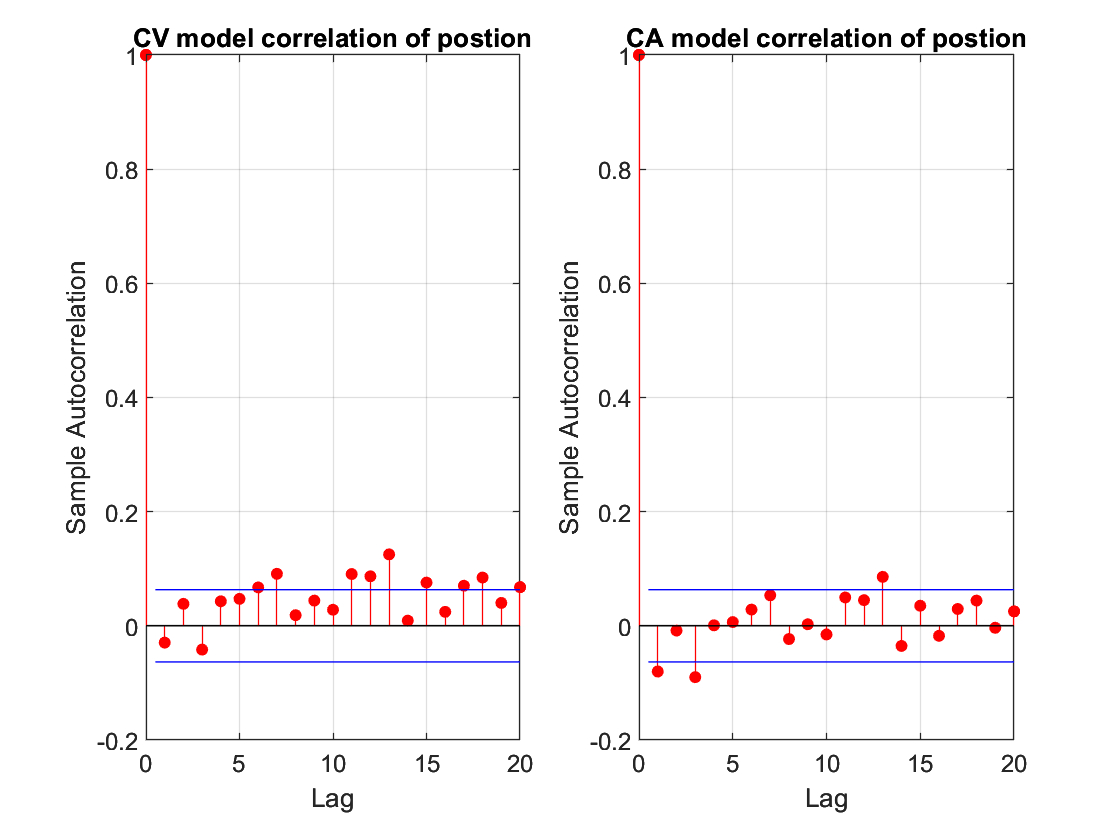
\includegraphics[width=0.7\textwidth]{images/correlationofposition.png}
 \caption{correlation of position}
 \label{2d1}
\end{figure}

\begin{figure}[H]
 \centering
 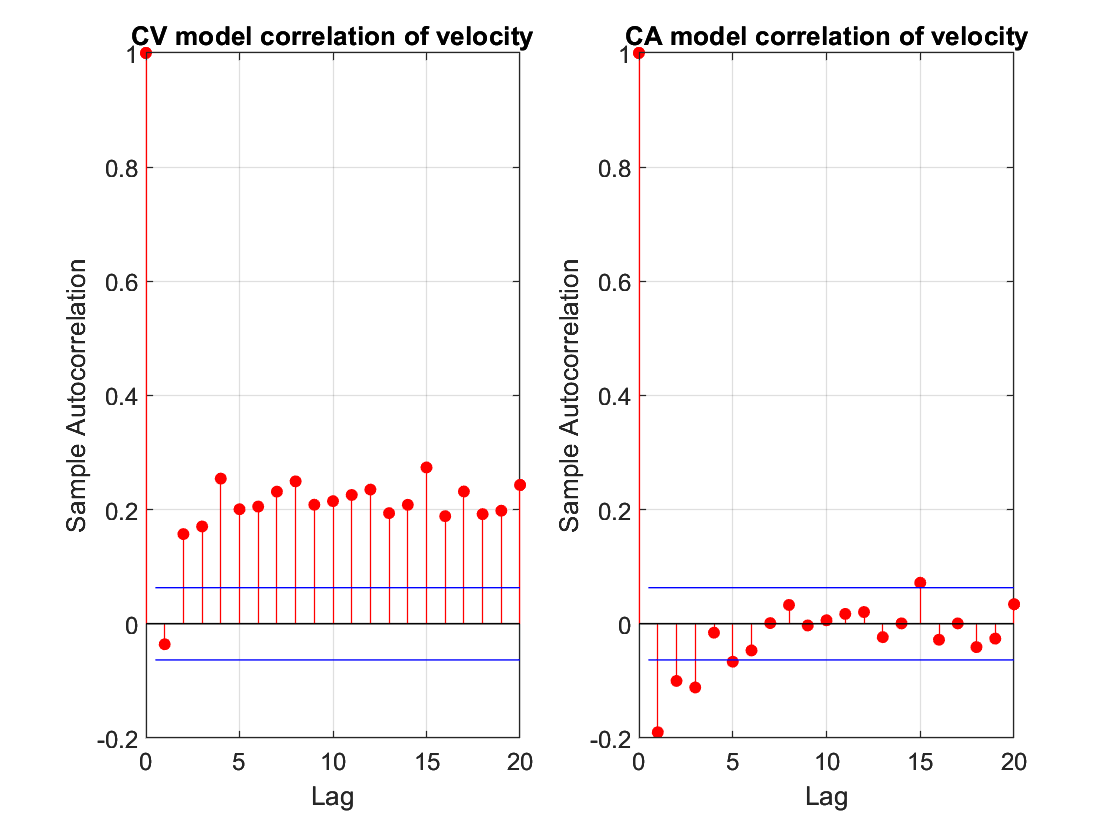
\includegraphics[width=0.7\textwidth]{images/correlationofvelocity.png}
 \caption{correlation of velocity}
 \label{2d2}
\end{figure}

Overall, the choice of the appropriate model depends on the specific scenario being considered and the assumptions made about the object being tracked. For our specific scenario, we should use \texttt{CA model}.